\documentclass{standalone}
\usepackage[T1]{fontenc}
\usepackage[x11names]{xcolor}
\usepackage{tikz}
\usepackage{pgfplots}
\usepackage{pgfplotstable}
\usepackage{filecontents}
\usepackage[osf,sc]{mathpazo}

\usetikzlibrary{shapes.geometric, arrows, intersections, through}
\usetikzlibrary{arrows.meta}

\newcommand\gauss[2]{1/(#2*sqrt(2*pi))*exp(-((x-#1)^2)/(2*#2^2))} 

\begin{document}
\pagestyle{empty}

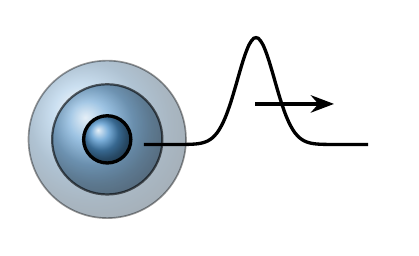
\begin{tikzpicture}[scale=1]
\shadedraw[semithick, ball color = SteelBlue3!100!white,opacity=0.4] (-0.18,0.2) circle (1);
\shadedraw[thick, ball color = SteelBlue3!100!white, opacity=0.6] (-0.18,0.2) circle (0.7);
\shadedraw[very thick, ball color = SteelBlue3!100!white] (-0.18,0.2) circle (0.3);
\draw[very thick, -{Stealth[scale=1.0]}] (1.7,0.65) -- (2.7,0.65);
%\draw[very thick, -{Stealth[scale=1.0]}] (-1.3,0.5) -- (-0.7,0.5);
%%\draw[very thick, -{Stealth[scale=1.0]}] (0.9,0.65) -- (1.8,0.65);
%%\draw[very thick, -{Stealth[scale=1.0]}] (0.9,0.65) -- (1.8,0.65);
\draw (1,-0.5) node[below,white]{\scriptsize APECSS};
\begin{axis}[width=5cm,height=3.2cm, every axis plot post/.append style={
  mark=none,domain=-2:2,samples=50,smooth}, 
axis line style={draw=none}, tick style={draw=none},xticklabels=\empty, yticklabels=\empty] 
\addplot[very thick, black] {\gauss{0}{0.33}};
\end{axis}
\end{tikzpicture}


%\begin{tikzpicture}[scale=1]
%\shadedraw[very thick, ball color = SkyBlue2!100!white] (0,0) circle (1);
%\draw[very thick, black] ((0.7,0) sin (1.2,0.5) cos (1.7,0);
%\addplot {\gauss{0}{0.5}}
%%\draw[-{Stealth[scale=1.1]}] (0,0) -- (-0.5,0.5);
%%\draw (-0.13,0.17) node[above]{\scriptsize $R$};
%%\draw[black,fill=black] (0,0) circle (0.04);
%%\draw (0,-0.1) node[below]{\scriptsize $p^{(2)}$};
%%\draw (0.75,0.75) node{\scriptsize $p^{(1)}$};
%%\draw (0.75,-0.6) node{\scriptsize $\sigma$};
%%\draw (0.5,-0.5) -- (0.67,-0.58);
%%\draw[black,fill=white] (0.5,-0.5) circle (0.025);
%%\draw (1.52,0) node[below]{\scriptsize $r$};
%\end{tikzpicture}
\end{document}